\documentclass[11pt]{beamer}

\usetheme[sectionpages,logo={_figures/poli-blue.pdf}]{UniNA}
\usefonttheme[onlymath]{serif}

\usepackage{tikz}
\usepackage{graphicx}
\usepackage{caption}
\usepackage{subcaption}
\usepackage{stanli}
\usepackage{siunitx}
\usepackage{mathtools}
\usepackage{quotes}
\usepackage{amsmath}
\usepackage{empheq}

\title{Sistema de suspensão rocker-bogie} %shown in title frame
\subtitle{PEF-3208 - Fundamentos em Mecânica das Estruturas}  % could also be a conference name

\date{\today} %explicitly set date instead of \today

\author[Natanael M. Cardoso]{Natanael Magalhães Cardoso}

\institute{Escola Politécnica - Universidade de São Paulo}

\begin{document}

\maketitle

\section{Introdução}

\begin{frame}{Sobre o sistema rocker-bogie}
  \begin{columns}
    \column{.59\textwidth}
    \begin{itemize}
      \item Desenvolvido em 1988 para o uso da NASA na exploração de Marte.
      \item Usado para movimentar robôs de 6 rodas.
    \end{itemize}
    \column{.39\textwidth}
    \begin{figure}[ht]
      \centering
      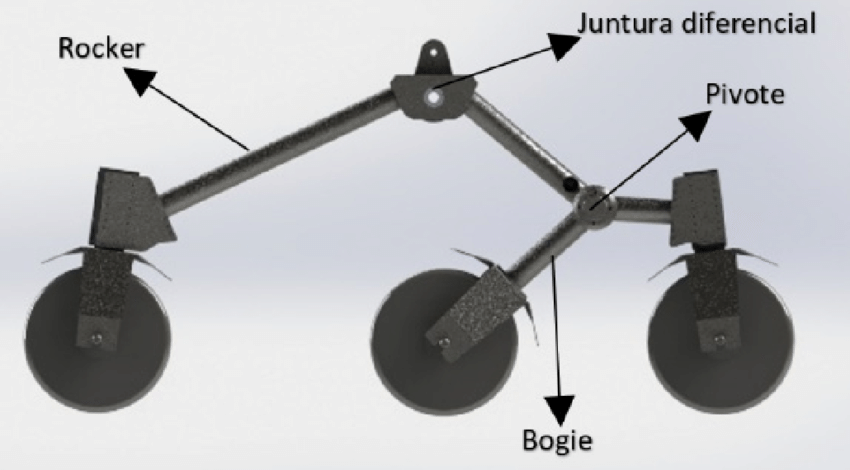
\includegraphics[width=.9\textwidth]{fig/rb-suspension.png}
    \end{figure}
    \vspace{5mm}
    \begin{figure}[ht]
      \centering
      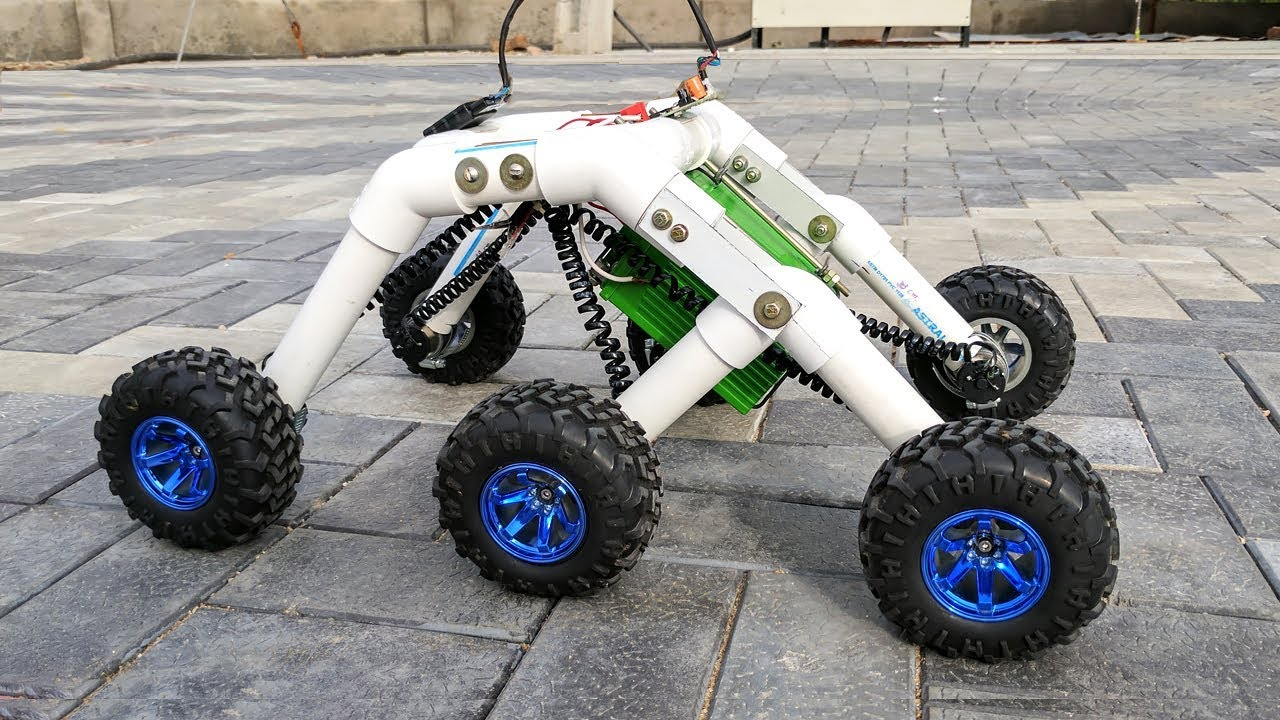
\includegraphics[width=.9\textwidth]{fig/rb.jpg}
    \end{figure}
  \end{columns}
\end{frame}

\end{document}